\documentclass[10pt]{article}
\usepackage{graphicx}
\graphicspath{ {img.jpg} }
\usepackage[margin=1in]{geometry} 
\usepackage{amsmath,amsthm,amssymb, graphicx, multicol, array}
 
\newcommand{\N}{\mathbb{N}}
\newcommand{\Z}{\mathbb{Z}}
 
\newenvironment{problem}[2][Problem]{\begin{trivlist}
\item[\hskip \labelsep {\bfseries #1}\hskip \labelsep {\bfseries #2.}]}{\end{trivlist}}



\begin{document}
\title{Problem Set 6}
\author{Hoang Nguyen, Huy Nguyen}
\maketitle
    
\begin{problem}{1}
\item 1.
Because $X_1, X_2,...X_n$ follow exponential, hence $\mathbb{E}[X]=\frac{1}{\lambda}$ and $\mathbb{V}[X]=\frac{1}{\lambda^2}$.\\
From CTT, we know: $\frac{\bar{X_n-\frac{1}{\lambda}}}{\frac{1}{\lambda}} \sim N(0,1)$.\\
Under $H_0$: $\frac{\bar{X_n-\frac{1}{\lambda_0}}}{\frac{1}{\lambda_0}} \sim N(0,1)$. Now we have test statistic: $T= |\frac{\bar{X_n-\frac{1}{\lambda_0}}}{\frac{1}{\lambda_0}}|$.\\
With asymptotic level $\alpha$, $\mathbb{P}[T>c]=\alpha$, hence $c=1-\phi^{-1}(\frac{\alpha}{2})$\\
Conclusion: If $T>c$, we reject $H_0$. Otherwise, we fail to reject $H_0$.


\item 2. 
Let denote $\hat{\lambda}=argmax_{\theta \in \{0; +\infty\}} l(\theta)$ and $\hat{\lambda^c}=argmax_{\theta \in H_0} l(\theta)$ where $l(\theta)$ is likehood funtion of $\theta$. Using Likelood ratio test, we have test stattistic: $T=2\Big(l(\hat{\lambda})-l(\hat{\lambda^c})\Big)$. \\
The difference in the number of parameters for the two models is 1 because we only consider paramer $\lambda \in \mathbb{R}$. Hence $T \sim \chi_{1}^{2}$. With asymptotic level test $\alpha$, $\mathbb{P}[T>c]=\alpha$, hence c is the $(1-\alpha)$-quantile of $\chi^{2}_{1}$.
Conclusion: If $T>c$, we reject $H_0$. Otherwise, we fail to reject $H_0$.

\item 3.
a) Because $X_1, X_2,...X_n$ follow exponential, hence $\l(\lambda)=nln(\lambda)- \lambda \sum_{i=1}^{n}X_i$. Because there are 50 consecutive calls and these observations have average value is 0.98, hence $ \sum_{i=1}^{n}X_i=0.98x50=49$.\\
Now we have log-likelihood function $l(\lambda)=50ln(\lambda)- 49\lambda$. Taking derivate respect to $\lambda$, we get $l'(\lambda)= \frac{50}{\lambda}-49$. Setting this equals to zeros we get $\hat{\lambda}=\frac{50}{49}$, hence $l(\hat{\lambda})=-48.989$\\
Because $l'(\lambda) > 0$ for all $\theta$ under $H_0$, hence $\hat{\lambda^c}=1 => l(\hat{\lambda^c})=-49$\\
Based on previous questions, we have $T=2\Big(l(\hat{\lambda})-l(\hat{\lambda^c})\Big)= 2(-48.989+49)=0.022$. With asymptotic level test $\alpha=0.05$, we get $c=3.814$\\
Because $T=0.022<3.814$, hence we fail to reject null hypothesis.\\
b) $p-value=\mathbb{P}[\chi_{1}^{2}>0.022]=0.8829$




















\end{problem}

\begin{problem}{2}
\item 1.
Take derivative of Gaussian expression respect to $\mu_1, \sigma_1,$ and set it equals to 0, we get:\\
$\hat{\mu}=\bar{X_{n}}$ and $\hat{\sigma}^2=\frac{1}{n}\sum_{i=1}^{n} (X_i-\hat(\mu))^2$.

\item 2.
Cochran’s theorem implies that for $X_1, X_2,...X_n$ follow Gaussian distribution with $\mu$ and $\sigma^2$, we have: 
\[\sqrt{n-1}\frac{\bar{X_n}-\mu}{\sqrt{S_n}} \sim t_{n-1} \]
From previous question, we have $\hat{\mu}=\bar{X_{n}}$ and $S_n=\hat{\sigma}^2=\frac{1}{n}\sum_{i=1}^{n} (X_i-\mu)^2$. Plugging this to the equation above, we get:
\[S=\sqrt{n-1}\frac{\hat{\mu}- \mu}{\sqrt{\hat{\sigma}^2}} \sim t_{n-1} \] 

\item 3 
From previous question, we know $S \sim t_{n-1}$, so we will bulid Student test based on this intuition with test statistic S.\\ 
Let denote $c$ is the ($1-\alpha$)-quantile of Student distribution with $n-1$ degrees of freedom. That means $\mathbb{P}[t_{n-1}> c]=\alpha$.\\
Based on the previous question, we have test statistic: $T=\sqrt{n-1}\frac{\hat{\mu}}{\sqrt{\hat{\sigma}^2}}= \sqrt{n-1}\frac{\bar{X_n}}{\sqrt{\frac{1}{n}\sum_{i=1}^{n} (X_i-\bar{X_n})^2}} \sim t_{n-1}$. Concretely, the graph below show the t-test diagram with Student test (n-1 dgrees of freedom) and level test $\alpha=0.05$, for example. 

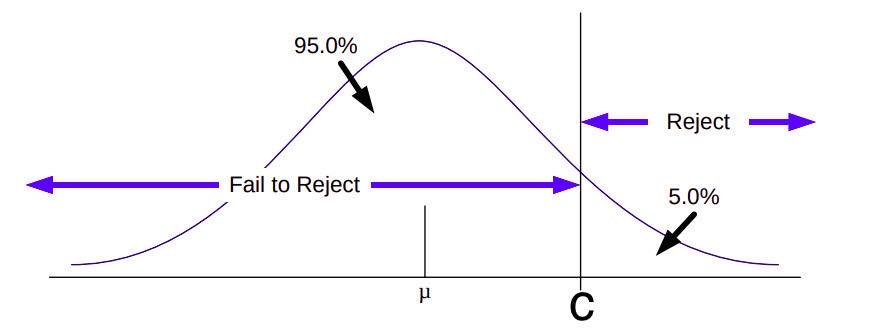
\includegraphics[totalheight=5cm]{img.jpg}\\
Conclusion: If $T>c$ that means $H_0$ fall into reject region so we reject $H_0$,. Otherwise, we are fail to reject $H_0$














\end{problem}

\begin{problem}{3}
\item 1.\\
$\bullet$ Prove X and Y are independent implies $r=pq$:\\
From Bayes rule, we have $\mathbb{P}[X=1|Y=1]=\frac{\mathbb{P}[X=1, Y=1]}{\mathbb{P}[Y=1]}$ (1) \\
From X and Y are independent, we have $\mathbb{P}[X=1|Y=1]=\mathbb{P}[X=1] $. Plugging this to (1), we have: 
$\mathbb{P}[X=1] \mathbb{P}[Y=1]=\mathbb{P}[X=1, Y=1] \Leftrightarrow r=pq$.\\
$\bullet$ Prove $r=pq$ implies X and Y are independent: \\
By defination of independent event, we have if $\mathbb{P}[X=1]\mathbb{P}[Y=1]=\mathbb{P}[X=1, Y=1] \Leftrightarrow r=pq$, X and Y are independent.\\
Hence X and Y are independent iff $r=pq$.
\item 2.\\
a)\\
$\bullet$ By Markov's inequality:
\[ \mathbb{P}\Big[|\hat{p} - p| > \epsilon \Big] \leqslant \mathbb{P}\Big[\hat{p} - p > \epsilon \Big] \leqslant \frac{\mathbb{E}[\hat{p}-p]}{\epsilon} = \frac{\mathbb{E}[\hat{p}]- p}{\epsilon}=0 \]
Hence, $\hat{p}$ is consistent estimators of $p$.\\
Using similar method, we get $\hat{q}$ and $\hat{r}$ are consistent estimator of q and r, respectively.\\
b)\\
From CTT, we have $\sqrt{n}\frac{\bar{X_n}-p}{\sqrt{p(1-p)}} \sim N(0,1) $. Hence, $\sqrt{n}(\hat{p}-p) \sim N(0, p(1-p))$. Using similar method, we get $\sqrt{n}(\hat{q}-q) \sim N(0, q(1-q))$ and $\sqrt{n}(\hat{r}-r) \sim N(0, r(1-r))$.\\
Hence, $(\hat{p}, \hat{q}, \hat{r})$ is asymptotically normal with covariance matrix 
\[ \Sigma
=
\begin{bmatrix}
    p(1-p) & 0 & 0\\
    0 & q(1-q) & 0\\
    0 & 0 & r(1-r)
\end{bmatrix} 
 \]
c)\\
From previous question we have: $\sqrt{n}(\hat{\theta} -\theta ) \sim N(0, \Sigma)$ where $\theta=\begin{bmatrix}
    r & p & q
    
\end{bmatrix}^{T}  $ and $\Sigma=\begin{bmatrix}
    r(1-r) & 0 & 0\\
    0 & p(1-p) & 0\\
    0 & 0 & q(1-q)
    
\end{bmatrix}  $\\
Let's denote $\theta= \begin{bmatrix}
    r & p & q
    
\end{bmatrix}^{T} $, $\hat{\theta}= \begin{bmatrix}
    \hat{r} & \hat{p} & \hat{q}
    
\end{bmatrix}^{T} $ and function $\mathbb{R}^3 \rightarrow \mathbb{R}: f(\theta)=\theta_1-\theta_2\theta_3$.\\
We have $\sqrt{n}(\hat{r}-\hat{p}\hat{q})=\sqrt{n}(f(\hat{\theta})-f(\theta))$ where $\theta=\begin{bmatrix}
    r & p & q
    
\end{bmatrix}^{T}  $. Using Delta-method we have:
\[ \sqrt{n}(f(\hat{\theta})-f(\theta)) \sim N(0, \nabla_{\theta}^{T} \Sigma \nabla_{\theta} ) \]
Where $\nabla_{\theta}=\frac{\partial f}{\partial \theta}(\theta)$ and $\Sigma$ is the covariance matrix of asymptotically normal distributiion of $\theta$. With  $\theta=\begin{bmatrix}
    r & p & q
    
\end{bmatrix}^{T}  $ we have: \[ \nabla_{\theta}= \frac{\partial f}{\partial \theta}(\theta)= 
\theta=\begin{bmatrix}
    1 & -q & -p
    
\end{bmatrix}^{T}
  \]
Hence $V=\nabla_{\theta}^{T} \Sigma \nabla_{\theta}=\begin{bmatrix}
    1 & -q & -p
    
\end{bmatrix} \begin{bmatrix}
    r(1-r) & 0 & 0\\
    0 & p(1-p) & 0\\
    0 & 0 & q(1-q)
    
\end{bmatrix}  \begin{bmatrix}
    1 \\
    -q\\
    -p\\
\end{bmatrix}=$.

\end{problem}

\end{document}